\let\negmedspace\undefined
\let\negthickspace\undefined
\documentclass[journal,12pt,onecolumn]{IEEEtran}
\usepackage{cite}
\usepackage{amsmath,amssymb,amsfonts,amsthm}
\usepackage{algorithmic}
\usepackage{graphicx}
\graphicspath{{./figs/}} 
\usepackage{textcomp}
\usepackage{xcolor}
\usepackage{txfonts}
\usepackage{listings}
\usepackage{enumitem}
\usepackage{mathtools}
\usepackage{gensymb}
\usepackage{comment}
\usepackage{caption}
\usepackage[breaklinks=true]{hyperref}
\usepackage{tkz-euclide} 
\usepackage{listings}
\usepackage{gvv}                                        
%\def\inputGnumericTable{}                                 
\usepackage[latin1]{inputenc}     
\usepackage{xparse}
\usepackage{color}                                            
\usepackage{array}                                            
\usepackage{longtable}                                       
\usepackage{calc}                                             
\usepackage{multirow}
\usepackage{multicol}
\usepackage{hhline}                                           
\usepackage{ifthen}                                           
\usepackage{lscape}
\usepackage{tabularx}
\usepackage{array}
\usepackage{float}
\newtheorem{theorem}{Theorem}[section]
\newtheorem{problem}{Problem}
\newtheorem{proposition}{Proposition}[section]
\newtheorem{lemma}{Lemma}[section]
\newtheorem{corollary}[theorem]{Corollary}
\newtheorem{example}{Example}[section]
\newtheorem{definition}[problem]{Definition}
\newcommand{\BEQA}{\begin{eqnarray}}
	\newcommand{\EEQA}{\end{eqnarray}}
\newcommand{\define}{\stackrel{\triangle}{=}}
\theoremstyle{remark}
\newtheorem{rem}{Remark}

\newcommand{\ihat}{\mathbf {\hat \imath}}
\newcommand{\jhat}{\mathbf {\hat \jmath}}
\newcommand{\vect}[1]{\mathbf #1}



\title{CH: CHEMICAL ENGINEERING}
\author{EE25BTECH11042 - Nipun Dasari}
\date{   }


\begin{document}
	
	\bibliographystyle{IEEEtran}
	\vspace{3cm}
	
	\maketitle
	\begin{enumerate}
		\item If $\to$ denotes increasing order of intensity, then the meaning of the words
		\brak{\text{simmer} \rightarrow \text{seethe} \rightarrow \text{smolder}} is analogous to \brak{\text{break} \to \text{raze} \to \underline{\hspace{2cm}}}
		Which one of the given options is appropriate to fill the blank?
		
		\hfill{\brak{\text{GATE CH 2024}}}
		\begin{enumerate}
			\begin{multicols}{2}
				\item obfuscate
				\item obliterate
				\item fracture
				\item fissure
			\end{multicols}
		\end{enumerate}
		
		\item In a locality, the houses are numbered in the following way: The house-numbers on one side of a road are consecutive odd integers starting from $301$, while the house-numbers on the other side of the road are consecutive even numbers starting from $302$. The total number of houses is the same on both sides of the road.
		If the difference of the sum of the house-numbers between the two sides of the road is $27$, then the number of houses on each side of the road is
		
		\hfill{\brak{\text{GATE CH 2024}}}
		\begin{enumerate}
			\item $27$
			\item $52$
			\item $54$
			\item $26$
		\end{enumerate}
		
		\item For $\frac{p}{q} \ne 1$ with P\underline{\hspace{2cm}}
		Then
		\begin{enumerate}
			\item $q^p = p^q$
			\item $q^p = p^{2q}$
			\item $\sqrt{q}=\sqrt{p}$
			\item $\sqrt[p]{q}=\sqrt[q]{p}$
		\end{enumerate}
		
		\hfill{\brak{\text{GATE CH 2024}}}
		
		\item Which one of the given options is a possible value of $x$ in the following sequence?
		$3, 7, 15, x, 63, 127, 255$
		
		\hfill{\brak{\text{GATE CH 2024}}}
		\begin{enumerate}
			\begin{multicols}{4}
				\item $35$
				\item $40$
				\item $45$
				\item $31$
			\end{multicols}
		\end{enumerate}
		
		\item On a given day, how many times will the second-hand and the minute-hand of a clock cross each other during the clock time $12 \colon 05 \colon 00$ hours to $12 \colon 55 \colon 00$ hours?
		
		\hfill{\brak{\text{GATE CH 2024}}}
		\begin{enumerate}
			\item $55$
			\item $12$
			\item $14$
			\item $10$
		\end{enumerate}
		
		\item In the given text, the blanks are numbered \brak{i}--\brak{iv}. Select the best match for all the blanks.
		From the ancient Athenian arena to the modern Olympic stadiums, \brak{i} the potential for a spectacle. The crowd \brak{ii} with bated breath as the Olympian artist twists his body, stretching the javelin behind him. Twelve strides in, he begins---an abrupt stop on his left foot. As his body \brak{iii} like a door turning on a hinge to cross-step. Six cross-steps in an instant, the javelin is launched skyward at \brak{iv}, a precise angle.
		
		\hfill{\brak{\text{GATE CH 2024}}}
		\begin{enumerate}
			\item \brak{i} holds \brak{ii} waits \brak{iii} culminates \brak{iv} pivots
			\item \brak{i} hold \brak{ii} wait \brak{iii} culminate \brak{iv} pivots
			\item \brak{i} hold \brak{ii} waits \brak{iii} culminate \brak{iv} pivot
			\item \brak{i} holds \brak{ii} wait \brak{iii} culminates \brak{iv} pivot
		\end{enumerate}
		
		\item Three distinct sets of indistinguishable twins are to be seated at a circular table that has $8$ identical chairs. Unique seating arrangements are defined by the relative positions of the people. How many unique seating arrangements are possible such that each person is sitting next to their twin?
		
		\hfill{\brak{\text{GATE CH 2024}}}
		\begin{enumerate}
			\begin{multicols}{4}
				\item $12$
				\item $14$
				\item $10$
				\item $28$
			\end{multicols}
		\end{enumerate}
		
		\item The chart given below compares the Installed Capacity \brak{\text{MW}} of four power generation technologies, $T1, T2, T3,$ and $T4$, and their Electricity Generation \brak{\text{MWh}} in a time of $1000$ hours \brak{\text{h}}.
		\begin{figure}
			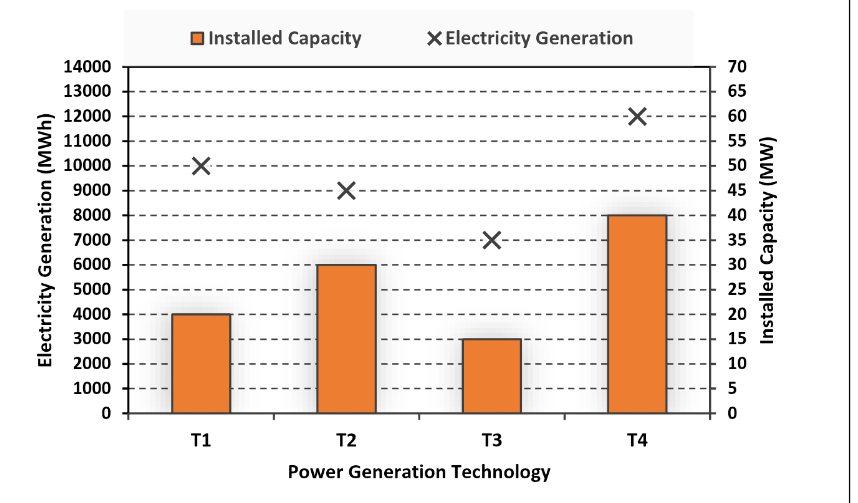
\includegraphics[width = 0.8\columnwidth]{q8}
			\caption*{}
			\label{fig:q8}
		\end{figure}
		The Capacity Factor of a power generation technology is:
		$$ \text{Capacity Factor} = \frac{\text{Electricity Generation}\brak{\text{MWh}}}{\text{Installed Capacity}\brak{\text{MW}}\times1000\brak{\text{h}}} $$
		Which one of the given technologies has the highest Capacity Factor?
		
		\hfill{\brak{\text{GATE CH 2024}}}
		\begin{enumerate}
			\item $T1$
			\item $T2$
			\item $T3$
			\item $T4$
		\end{enumerate}
		
		\item In the $4 \times 4$ array shown below, each cell of the first three columns has either a cross \brak{X} or a number, as per the given rule.
		\begin{figure}
			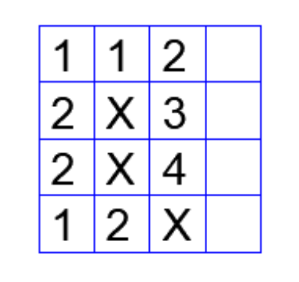
\includegraphics[width = 0.6\columnwidth]{q9}
			\caption*{}
			\label{fig:q9}
		\end{figure}
		Rule: The number in a cell represents the count of crosses around its immediate neighboring cells \brak{\text{left, right, top, bottom, diagonals}}.
		As per this rule, the maximum number of crosses possible in the empty column is
		
		\hfill{\brak{\text{GATE CH 2024}}}
		\begin{enumerate}
			\begin{multicols}{4}
				\item $0$
				\item $1$
				\item $2$
				\item $3$
			\end{multicols}
		\end{enumerate}
		
		\item During a half-moon phase, the Earth-Moon-Sun form a right triangle. If the Moon-Earth-Sun angle at this half-moon phase is measured to be $89.85\degree$, the ratio of the Earth-Sun and Earth-Moon distances is closest to
		
		\hfill{\brak{\text{GATE CH 2024}}}
		\begin{enumerate}
			\begin{multicols}{4}
				\item $328$
				\item $382$
				\item $238$
				\item $283$
			\end{multicols}
		\end{enumerate}

	
	
		\item The first non-zero term in the Taylor series expansion of $\brak{1-x}-e^{-x}$ about $x=0$ is
		
		\hfill{\brak{\text{GATE CH 2024}}}
		\begin{enumerate}
			\item $1$
			\item $-\frac{x^2}{2}$
			\item $\frac{x^2}{2}$
			\item $-1$
		\end{enumerate}
		
		\item Consider the normal probability distribution function
		$$ f\brak{x} = \frac{4}{\sqrt{2\pi}} e^{-8\brak{x+3}^2} $$
		If $\mu$ and $\sigma$ are the mean and standard deviation of $f\brak{x}$ respectively, then the ordered pair \brak{\mu, \sigma} is
		
		\hfill{\brak{\text{GATE CH 2024}}}
		\begin{enumerate}
			\item $\brak{3, \frac{1}{4}}$
			\item $\brak{-3, \frac{1}{4}}$
			\item \brak{3,4}
			\item \brak{-3,4}
		\end{enumerate}
		
		\item If $z_1 = -1+i$ and $z_2 = 2i$ where $i = \sqrt{-1}$, then $\text{Arg}\brak{z_1/z_2}$ is
		
		\hfill{\brak{\text{GATE CH 2024}}}
		\begin{enumerate}
			\begin{multicols}{4}
				\item $\frac{3\pi}{4}$
				\item $\frac{\pi}{4}$
				\item $\frac{\pi}{2}$
				\item $\frac{\pi}{3}$
			\end{multicols}
		\end{enumerate}
		
		\item A homogeneous azeotropic distillation process separates an azeotropic AB binary feed using a heavy entrainer, E, as shown in the figure. The loss of E in the two product streams is negligible so that E circulates around the process in a closed circuit. For a distillation column with fully specified feed\brak{s}, given operating pressure, a single distillate stream and a single bottoms stream, the steady-state degrees of freedom equals $2$. For the process in the figure with a fully specified AB feed stream and given column operating pressures, the steady-state degrees of freedom equals
		\begin{figure}
			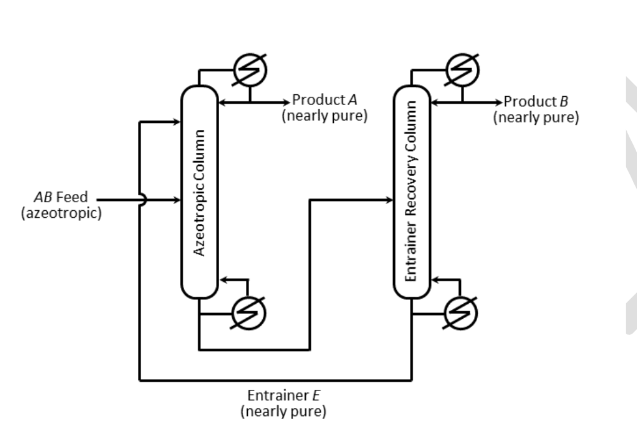
\includegraphics[width = 0.8\columnwidth]{q14}
			\caption*{}
			\label{fig:q14}
		\end{figure}
		
		\hfill{\brak{\text{GATE CH 2024}}}
		\begin{enumerate}
			\begin{multicols}{4}
				\item $3$
				\item $4$
				\item $5$
				\item $6$
			\end{multicols}
		\end{enumerate}
		
		\item An infinitely long cylindrical water filament of radius $R$ is surrounded by air. Assume water and air to be static. The pressure outside the filament is $P_{\text{out}}$ and the pressure inside is $P_{\text{in}}$. If $\gamma$ is the surface tension of the water-air interface, then $P_{\text{in}} - P_{\text{out}}$ is
		
		\hfill{\brak{\text{GATE CH 2024}}}
		\begin{enumerate}
			\begin{multicols}{4}
				\item $\frac{2\gamma}{R}$
				\item $0$
				\item $\frac{\gamma}{R}$
				\item $\frac{4\gamma}{R}$
			\end{multicols}
		\end{enumerate}
		
		\item The velocity field in an incompressible flow is $\boldsymbol{v} = \alpha x y \hat{\boldsymbol{i}} + v_y \hat{\boldsymbol{j}} + \beta \hat{\boldsymbol{k}}$, where $\hat{\boldsymbol{i}}, \hat{\boldsymbol{j}}$ and $\hat{\boldsymbol{k}}$ are unit-vectors in the \brak{x, y, z} Cartesian coordinate system. Given that $\alpha$ and $\beta$ are constants, and $v_y = 0$ at $y=0$, the correct expression for $v_y$ is
		
		\hfill{\brak{\text{GATE CH 2024}}}
		\begin{enumerate}
			\begin{multicols}{4}
				\item $-\alpha x y^2$
				\item $-\frac{\alpha y^2}{2}$
				\item $\frac{\alpha y^2}{2}$
				\item $\frac{\alpha x y}{2}$
			\end{multicols}
		\end{enumerate}
		
		\item Consider the steady, uni-directional diffusion of a binary mixture of $A$ and $B$ across a vertical slab of dimensions $0.2$ m $\times$ $0.1$ m $\times$ $0.02$ m as shown in the figure. The total molar concentration of $A$ and $B$ is constant at $100$ mol m$^{-3}$. The mole fraction of $A$ on the left and right faces of the slab are maintained at $0.8$ and $0.2$, respectively. If the binary diffusion coefficient $D_{AB} = 1 \times 10^{-5}$ m$^2$s$^{-1}$, the molar flow rate of $A$ in mol s$^{-1}$, along the horizontal $x$ direction is
		\begin{figure}
			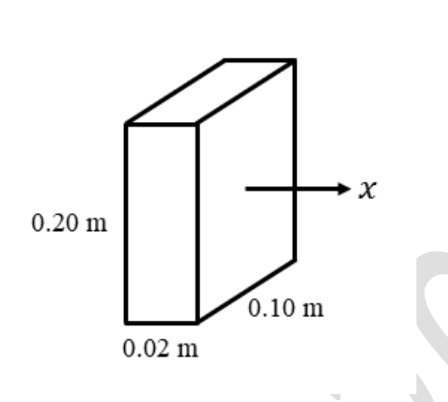
\includegraphics[width = 0.5\columnwidth]{q17}
			\caption*{}
			\label{fig:q17}
		\end{figure}
		
		\hfill{\brak{\text{GATE CH 2024}}}
		\begin{enumerate}
			\begin{multicols}{4}
				\item $6 \times 10^{-4}$
				\item $6 \times 10^{-6}$
				\item $3 \times 10^{-6}$
				\item $3 \times 10^{-4}$
			\end{multicols}
		\end{enumerate}
		
		\item A vapour-liquid mixture of components $A$ and $B$ obeys Raoult's law. The vapour pressure of $A$ is half that of $B$. The vapour phase concentrations of $A$ and $B$ are $3$ mol m$^{-3}$ and $6$ mol m$^{-3}$, respectively. At equilibrium, the ratio of the liquid phase concentration of $A$ to that of $B$ is
		
		\hfill{\brak{\text{GATE CH 2024}}}
		\begin{enumerate}
			\begin{multicols}{4}
				\item $1.0$
				\item $0.5$
				\item $2.0$
				\item $1.5$
			\end{multicols}
		\end{enumerate}
		
		\item The ratio of the activation energy of a chemical reaction to the universal gas constant is $1000$ K. The temperature-dependence of the reaction rate constant follows the collision theory. The ratio of the rate constant at $600$ K to that at $400$ K is
		
		\hfill{\brak{\text{GATE CH 2024}}}
		\begin{enumerate}
			\begin{multicols}{4}
				\item $2.818$
				\item $4.323$
				\item $1.502$
				\item $1.000$
			\end{multicols}
		\end{enumerate}
		
		\item The rate of a reaction $A \to B$ is $0.2$ mol m$^{-3}$s$^{-1}$ at a particular concentration $C_{A1}$. The rate constant of the reaction at a given temperature is $0.1$ m$^3$ mol$^{-1}$s$^{-1}$. If the reactant concentration is increased to $10 C_{A1}$ at the same temperature, the reaction rate, in mol m$^{-3}$s$^{-1}$, is
		
		\hfill{\brak{\text{GATE CH 2024}}}
		\begin{enumerate}
			\begin{multicols}{4}
				\item $20$
				\item $10$
				\item $100$
				\item $50$
			\end{multicols}
		\end{enumerate}
		
		\item Two parallel first-order liquid phase reactions $A \xrightarrow{k_1} B$ and $A \xrightarrow{k_2} C$ are carried out in a well-mixed isothermal batch reactor. The initial concentration of $A$ in the reactor is $1$ kmol m$^{-3}$, while that of $B$ and $C$ is zero. After $2$ hours, the concentration of $A$ reduces to half its initial value, and the concentration of $B$ is twice that of $C$. The rate constants $k_1$ and $k_2$, in h$^{-1}$, are, respectively
		
		\hfill{\brak{\text{GATE CH 2024}}}
		\begin{enumerate}
			\begin{multicols}{4}
				\item $0.40, 0.20$
				\item $0.23, 0.12$
				\item $0.50, 0.25$
				\item $0.36, 0.18$
			\end{multicols}
		\end{enumerate}
		
		\item Consider the block diagram in the figure with control input $u$, disturbance $d$ and output $y$. For the feedforward controller, the ordered pair $\brak{K, \alpha\beta}$ is
		\begin{figure}
			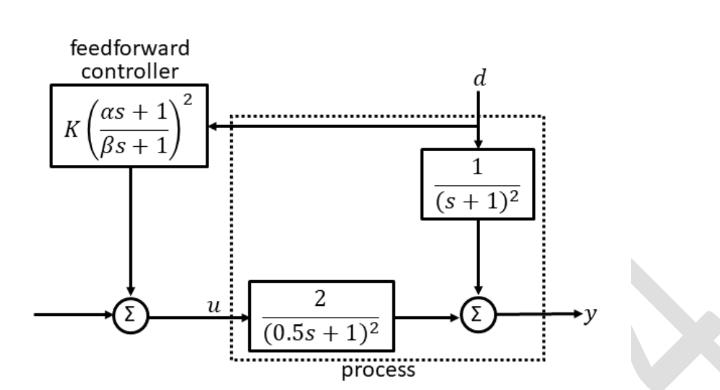
\includegraphics[width = 0.7\columnwidth]{q22}
			\caption*{}
			\label{fig:q22}
		\end{figure}
		
		\hfill{\brak{\text{GATE CH 2024}}}
		\begin{enumerate}
			\begin{multicols}{4}
				\item \brak{0.5, 2}
				\item \brak{-0.5, 0.5}
				\item \brak{-2, 2}
				\item \brak{2, 0.5}
			\end{multicols}
		\end{enumerate}
		
		\item Consider the control structure for the overhead section of a distillation column shown in the figure. The composition controller \brak{CC} controls the heavy key impurity in the distillate by adjusting the setpoint of the reflux flow controller in a cascade arrangement. The sign of the controller gain for the pressure controller \brak{PC} and that for the composition controller \brak{CC} are, respectively,
		\begin{figure}
			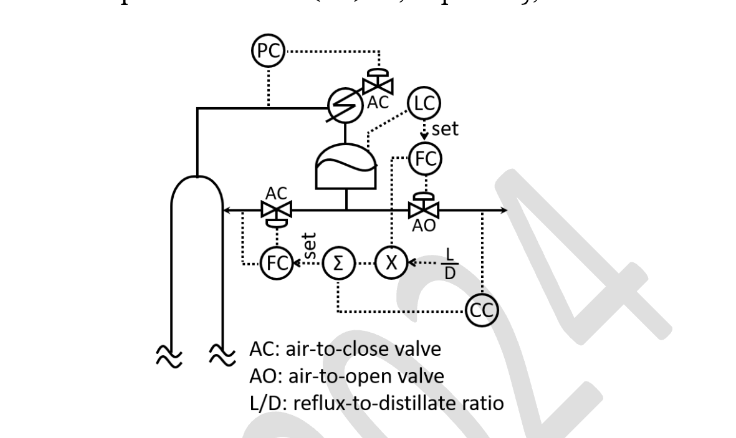
\includegraphics[width = 0.8\columnwidth]{q23}
			\caption*{}
			\label{fig:q23}
		\end{figure}
		
		\hfill{\brak{\text{GATE CH 2024}}}
		\begin{enumerate}
			\item negative, negative
			\item negative, positive
			\item positive, positive
			\item positive, negative
		\end{enumerate}
		
		\item Which one of the given statements is correct with reference to gas-liquid contactors for mass transfer applications?
		
		\hfill{\brak{\text{GATE CH 2024}}}
		\begin{enumerate}
			\item A tray tower is more suitable for foaming systems than a packed tower.
			\item Tray towers are preferred over packed towers for systems requiring frequent cleaning.
			\item For a given liquid flow rate, the gas flow rate in the loading region is greater than that in the flooding region.
			\item Flooding can never occur for counter-current contact.
		\end{enumerate}
		
		\item In an ammonia manufacturing facility, the necessary hydrogen is generated from methane. The facility consists of the following process units - P: Methanator, Q: CO shift convertor, R: CO$_2$ stripper, S: Reformer, T: Ammonia convertor. The correct order of these units, starting from methane feed is
		
		\hfill{\brak{\text{GATE CH 2024}}}
		\begin{enumerate}
			\item S, Q, R, P, T
			\item P, Q, R, S, T
			\item S, P, Q, R, T
			\item P, S, T, Q, R
		\end{enumerate}
		
		\item Consider a linear homogeneous system of equations $\vec{A}\vec{x} = \vec{0}$, where $\vec{A}$ is an $n \times n$ matrix, $\vec{x}$ is an $n \times 1$ vector and $\vec{0}$ is an $n \times 1$ null vector. Let $r$ be the rank of $\vec{A}$. For a non-trivial solution to exist, which of the following conditions is/are satisfied?
		
		\hfill{\brak{\text{GATE CH 2024}}}
		\begin{enumerate}
			\item Determinant of $\vec{A} = 0$
			\item $r=n$
			\item $r < n$
			\item Determinant of $\vec{A} \ne 0$
		\end{enumerate}
		
		\item If the Prandtl number $\text{Pr} = 0.01$, which of the following statements is/are correct?
		
		\hfill{\brak{\text{GATE CH 2024}}}
		\begin{enumerate}
			\item The momentum diffusivity is much larger than the thermal diffusivity.
			\item The thickness of the momentum boundary layer is much smaller than that of the thermal boundary layer.
			\item The thickness of the momentum boundary layer is much larger than that of the thermal boundary layer.
			\item The momentum diffusivity is much smaller than the thermal diffusivity.
		\end{enumerate}
		
		\item For the electrolytic cell in a chlor-alkali plant, which of the following statements is/are correct?
		
		\hfill{\brak{\text{GATE CH 2024}}}
		\begin{enumerate}
			\item A membrane cell operates at a higher brine concentration than a diaphragm cell.
			\item Chlorine gas is produced at the cathode.
			\item Hydrogen gas is produced at the cathode.
			\item The caustic product stream exits the cathode compartment.
		\end{enumerate}
		
		\item Which of the following statements with reference to the petroleum/petrochemical industry is/are correct?
		
		\hfill{\brak{\text{GATE CH 2024}}}
		\begin{enumerate}
			\item Catalytic hydrocracking converts heavier hydrocarbons to lighter hydrocarbons.
			\item Catalytic reforming converts straight-chain hydrocarbons to aromatics.
			\item Cumene is manufactured by the catalytic alkylation of benzene with propylene.
			\item Vinyl acetate is manufactured by reacting methane with acetic acid over a palladium catalyst.
		\end{enumerate}
		
		\item Consider a matrix $\vec{A} = \myvec{-5 & a-2 \\ a-2 & -2}$, where $a$ is a constant. If the eigenvalues of $A$ are $-1$ and $-6$, then the value of $a$, rounded off to the nearest integer, is \underline{\hspace{2cm}}
		
		\hfill{\brak{\text{GATE CH 2024}}}
		
		\item Consider the reaction $N_2\brak{g} + 3H_2\brak{g} \rightleftharpoons 2NH_3\brak{g}$ in a continuous flow reactor under steady-state conditions. The component flow rates at the reactor inlet are $F_{N_2,0} = 100$ mol s$^{-1}$, $F_{H_2,0} = 300$ mol s$^{-1}$, $F_{\text{inert},0} = 1$ mol s$^{-1}$. If the fractional conversion of $H_2$ is $0.60$, the outlet flow rate of $N_2$, in mol s$^{-1}$, rounded off to the nearest integer, is \underline{\hspace{2cm}}
		
		\hfill{\brak{\text{GATE CH 2024}}}
		
		\item Consider a binary mixture of components $A$ and $B$ at temperature $T$ and pressure $P$. Let $\bar{V}_A$ and $\bar{V}_B$ be the partial molar volumes of $A$ and $B$, respectively. At a certain mole fraction of $A$, $x_A$ $\brak{\frac{\partial \bar{V}_A}{\partial x_A}}_{T,P} = 22$ cm$^3$ mol$^{-1}$ and $\brak{\frac{\partial \bar{V}_B}{\partial x_A}}_{T,P} = -18$ cm$^3$ mol$^{-1}$ The value of $x_A$, rounded off to 2 decimal places, is \underline{\hspace{2cm}}
		
		\hfill{\brak{\text{GATE CH 2024}}}
		
		\item Consider the steady, uni-directional, fully-developed, pressure-driven laminar flow of an incompressible Newtonian fluid through a circular pipe of inner radius $5.0$ cm. The magnitude of shear stress at the inner wall of the pipe is $0.1$ N m$^{-2}$. At a radial distance of $1.0$ cm from the pipe axis, the magnitude of the shear stress, in N m$^{-2}$, rounded off to 3 decimal places, is \underline{\hspace{2cm}}
		
		\hfill{\brak{\text{GATE CH 2024}}}
		
		\item The opposite faces of a metal slab of thickness $5$ cm and thermal conductivity $400$ W m$^{-1}$ \degree C$^{-1}$ are maintained at $500$ \degree C and $200$ \degree C. The area of each face is $0.02$ m$^2$. Assume that the heat transfer is steady and occurs only in the direction perpendicular to the faces. The magnitude of the heat transfer rate, in kW, rounded off to the nearest integer, is \underline{\hspace{2cm}}
		
		\hfill{\brak{\text{GATE CH 2024}}}
		
		\item The capital cost of a distillation column is Rs. $90$ lakhs. The cost is to be fully depreciated \brak{\text{salvage value is zero}} using the double-declining balance method over $10$ years. At the end of two years of continuous operation, the book-value of the column, in lakhs of rupees, rounded off to 1 decimal place, is \underline{\hspace{2cm}}
		
		\hfill{\brak{\text{GATE CH 2024}}}
		
		\item Consider a steady, fully-developed, uni-directional laminar flow of an incompressible Newtonian fluid \brak{viscosity \mu} between two infinitely long horizontal plates separated by a distance $2H$ as shown in the figure. The flow is driven by the combined action of a pressure gradient and the motion of the bottom plate at $y=-H$ in the negative $x$ direction. Given that $\frac{\Delta P}{L} = \brak{\frac{P_1-P_2}{L}} > 0$, where $P_1$ and $P_2$ are the pressures at two $x$ locations separated by a distance $L$.
	\begin{figure}
		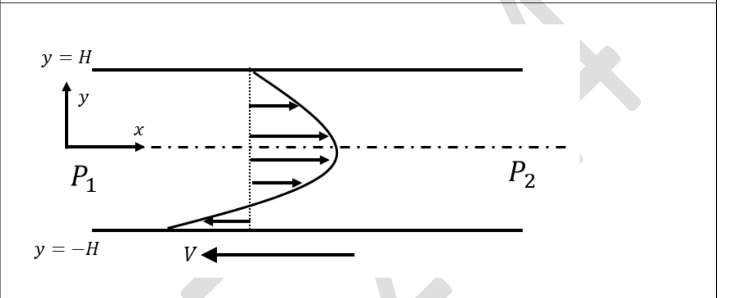
\includegraphics[width = 0.8\columnwidth]{q36}
		\caption*{}
		\label{fig:q36}
	\end{figure}
	\hfill{\brak{\text{GATE CH 2024}}}
	

	\begin{enumerate}
		\item $\frac{\Delta P}{L}\frac{H^{2}}{2\mu}\brak{1-\frac{y^{2}}{H^{2}}}+\frac{V}{2}\brak{\frac{y}{H}-1}$
		\item $\frac{\Delta P}{L}\frac{H^{2}}{2\mu}\brak{\frac{y^{2}}{H^{2}}-1}+\frac{V}{2}\brak{\frac{y}{H}-1}$
		\item $\frac{\Delta P}{L}\frac{H^{2}}{2\mu}\brak{\frac{y^{2}}{H^{2}}-1}-\frac{V}{2}\brak{\frac{y}{H}-1}$
		\item $\frac{\Delta P}{L}\frac{H^{2}}{2\mu}\brak{1-\frac{y^{2}}{H^{2}}}-\frac{V}{2}\brak{\frac{y}{H}-1}$
	\end{enumerate}
	
	\item The temperatures of two large parallel plates of equal emissivity are $900$ K and $300$ K. A reflection radiation shield of low emissivity and negligible conductive resistance is placed parallelly between them. The steady-state temperature of the shield, in K, is
	
	\hfill{\brak{\text{GATE CH 2024}}}
	\begin{enumerate}
		\item $759$
		\item $559$
		\item $659$
		\item $859$
	\end{enumerate}
	
	\item Hot oil at $110\degree$C heats water from $30\degree$C to $70\degree$C in a counter-current double-pipe heat exchanger. The flow rates of water and oil are $50$ kg min$^{-1}$ and $100$ kg min$^{-1}$, respectively and their specific heat capacities are $4.2$ kJ kg$^{-1}\degree$C$^{-1}$ and $2.0$ kJ kg$^{-1}\degree$C$^{-1}$ respectively. Assume the heat exchanger is at steady state. If the overall heat transfer coefficient is $200$ W m$^{-2}\degree$C$^{-1}$, the heat transfer area in m$^2$ is
	
	\hfill{\brak{\text{GATE CH 2024}}}
	\begin{enumerate}
		\item $5.2$
		\item $1.1$
		\item $17.9$
		\item $35.2$
	\end{enumerate}
	
	\item A solid slab of thickness $H_1$ is initially at a uniform temperature $T_0$. At time $t=0$, the temperature of the top surface at $y=H_1$ is increased to $T_1$, while the bottom surface at $y=0$ is maintained at $T_0$ for $t\ge0$. Assume heat transfer occurs only in the $y$-direction, and all thermal properties of the slab are constant. The time required for the temperature at $y=H_1/2$ to reach $99\%$ of its final steady value is $\tau_1$. If the thickness of the slab is doubled to $H_2=2H_1$, and the time required for the temperature at $y=H_2/2$ to reach $99\%$ of its final steady value is $\tau_2$, then $\tau_2/\tau_1$ is
	
	\hfill{\brak{\text{GATE CH 2024}}}
	\begin{enumerate}
		\item $2$
		\item $\frac{1}{4}$
		\item $4$
		\item $\frac{1}{2}$
	\end{enumerate}
	
	\item A gas stream containing $95$ mol\% $CO_2$ and $5$ mol\% ethanol is to be scrubbed with pure water in a counter-current, isothermal absorption column to remove ethanol. The desired composition of ethanol in the exit gas stream is $0.5$ mol\%. The equilibrium mole fraction of ethanol in the gas phase, $y^*$, is related to that in the liquid phase, $x$, as $y^*=2x$. Assume $CO_2$ is insoluble in water and neglect evaporation of water. If the water flow rate is twice the minimum, the mole fraction of ethanol in the spent water is
	
	\hfill{\brak{\text{GATE CH 2024}}}
	\begin{enumerate}
		\item $0.0225$
		\item $0.0126$
		\item $0.0428$
		\item $0.0316$
	\end{enumerate}
	
	\item Sulfur dioxide $\brak{SO_2}$ gas diffuses through a stagnant air-film of thickness $2$ mm at $1$ bar and $30\degree$C. The diffusion coefficient of $SO_2$ in air is $1 \times 10^{-5}$ m$^2$s$^{-1}$. The $SO_2$ partial pressures at the opposite sides of the film are $0.15$ bar and $0.05$ bar. The universal gas constant is $8.314$ J mol$^{-1}$K$^{-1}$. Assuming ideal gas behavior, the steady-state flux of $SO_2$ in mol m$^{-2}$s$^{-1}$ through the air-film is
	
	\hfill{\brak{\text{GATE CH 2024}}}
	\begin{enumerate}
		\item $0.022$
		\item $0.085$
		\item $0.057$
	\end{enumerate}
	
	\item A simple distillation column separates a binary mixture of A and B. The relative volatility of A with respect to B is 2. The steady-state composition of A in the vapour leaving the $1^{\text{st}}$, $2^{\text{nd}}$ and $3^{\text{rd}}$ trays in the rectifying section are $94$, $90$ and $85$ mol\%, respectively. For ideal trays and constant molal overflow, the reflux-to-distillate ratio is
	
	\hfill{\brak{\text{GATE CH 2024}}}
	\begin{enumerate}
		\item $1.9$
		\item $2.7$
		\item $1.2$
		\item $1.1$
	\end{enumerate}
	
	\item Alumina particles with an initial moisture content of $5$ kg per kg dry solid are dried in a batch dryer. For the first two hours, the measured drying rate is constant at $2$ kg m$^{-2}$h$^{-1}$. Thereafter, in the falling-rate period, the rate decreases linearly with the moisture content. The equilibrium moisture content is $0.05$ kg per kg dry solid and the drying area of the particles is $0.5$ m$^2$ per kg dry solid. The total drying time, in h, to reduce the moisture content to half its initial value is
	
	\hfill{\brak{\text{GATE CH 2024}}}
	\begin{enumerate}
		\item $4.13$
		\item $2.55$
		\item $3.22$
		\item $5.13$
	\end{enumerate}
	
	\item A first-order heterogenous reaction $A \to B$ is carried out using a porous spherical catalyst. Assume isothermal conditions, and that intraphase diffusion controls the reaction rate. At a bulk A concentration of $0.3$ mol L$^{-1}$, the observed reaction rate in a $3$ mm diameter catalyst particle is $0.2$ mol s$^{-1}$L$^{-1}$ catalyst volume. At a bulk A concentration of $0.1$ mol L$^{-1}$, the observed reaction rate, in mol s$^{-1}$L$^{-1}$ catalyst volume, in a $6$ mm diameter catalyst particle, is
	
	\hfill{\brak{\text{GATE CH 2024}}}
	\begin{enumerate}
		\item $0.011$
		\item $0.033$
		\item $0.022$
		\item $0.005$
	\end{enumerate}
	
	\item A first-order liquid phase reaction $A \to B$ is carried out in two isothermal plug flow reactors \brak{PFRs} of volume $1$ m$^3$ each, connected in series. The feed flow rate and concentration of A to the first reactor are $10$ m$^3$ h$^{-1}$ and $1$ kmol m$^{-3}$, respectively. At steady-state, the concentration of A at the exit of the second reactor is $0.2$ kmol m$^{-3}$. If the two PFRs are replaced by two equal-volume continuously stirred tank reactors \brak{CSTRs} to achieve the same overall steady-state conversion, the volume of each CSTR, in m$^3$, is
	
	\hfill{\brak{\text{GATE CH 2024}}}
	\begin{enumerate}
		\item $1.54$
		\item $3.84$
		\item $7.28$
		\item $1.98$
	\end{enumerate}
	
	\item The residence time distribution, E, for a non-ideal flow reactor is given in the figure. A first-order liquid phase reaction with a rate constant $0.2$ min$^{-1}$ is carried out in the reactor. For an inlet reactant concentration of $2$ mol L$^{-1}$ the reactant concentration \brak{\text{in mol } L^{-1}} in the exit stream is
	\begin{figure}
		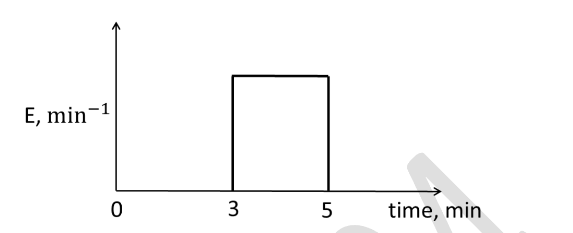
\includegraphics[width = 0.5\columnwidth]{q46}
		\caption*{}
		\label{fig:q46}
	\end{figure}
	
	\hfill{\brak{\text{GATE CH 2024}}}
	\begin{enumerate}
		\item $0.905$
		\item $0.452$
		\item $1.902$
	\end{enumerate}
	
	\item Let $r$ and $\theta$ be the polar coordinates defined by $x=r \cos \theta$ and $y=r \sin \theta$. The area of the cardioid $r=a\brak{1-\cos\theta}$, $0\le\theta\le2\pi,$ is
	
	\hfill{\brak{\text{GATE CH 2024}}}
	\begin{enumerate}
		\item $\frac{3\pi a^2}{2}$
		\item $\frac{2\pi a^2}{3}$
		\item $2\pi a^2$
		\item $3\pi a^2$
	\end{enumerate}
	
	\item For the block diagram shown in the figure, the correct expression for the transfer function $G_d=\frac{y_1\brak{s}}{d\brak{s}}$ is
	\begin{figure}
		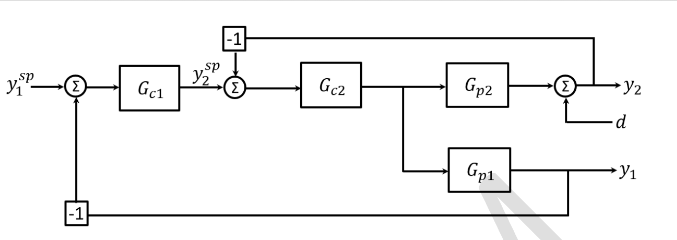
\includegraphics[width = 0.8\columnwidth]{q48}
		\caption*{}
		\label{fig:q48}
	\end{figure}
	
	\hfill{\brak{\text{GATE CH 2024}}}
	\begin{enumerate}
		\item $\frac{-G_{p1}G_{c2}}{\brak{1+G_{c1}G_{c2}G_{p1}}\brak{1+G_{c2}G_{p2}}}$
		\item $\frac{-G_{p1}G_{c2}}{1+G_{c2}G_{p2}+G_{c1}G_{c2}G_{p1}G_{p2}}$
		\item $\frac{-G_{p1}G_{c2}}{1+G_{c2}G_{p2}+G_{c1}G_{c2}G_{p1}}$
		\item $\frac{-G_{p1}}{1+G_{c2}G_{p2}+G_{c1}G_{c2}G_{p1}G_{p2}}$
	\end{enumerate}
	
	\item For purchasing a batch reactor, three alternatives P, Q and R have emerged, as summarized in the table. For a compound interest rate of $10\%$ per annum, choose the correct option that arranges the alternatives, in order, from the least expensive to the most expensive.
	\begin{table}
		\begin{tabular}{|c|c|c|c|}
			\hline
			& P & Q & R \\
			\hline
			Installed Cost \brak{\text{lakh rupees}} & $15$ & $25$ & $35$ \\
			\hline
			Equipment Life \brak{\text{years}} & $10$ & $3$ & $15$ \\
			\hline
			Maintenance Cost \brak{\text{lakh rupees per year}} & $0.5$ & $1.0$ & $0.2$ \\
			\hline
		\end{tabular}
		\caption*{}
		\label{tab:q49}
	\end{table}
	
	\hfill{\brak{\text{GATE CH 2024}}}
	\begin{enumerate}
		\item P, Q, R
		\item R, P, Q
		\item R, Q, P
		\item Q, P, R
	\end{enumerate}
	
	\item The Newton-Raphson method is used to solve $f\brak{x}=0$, where $f\brak{x}=e^x - 5x$. If the initial guess $x^{\brak{0}}=1.0$ the value of the next iterate, $x^{\brak{1}}$ rounded off to 2 decimal places, is \underline{\hspace{2cm}}
	
	\hfill{\brak{\text{GATE CH 2024}}}
	
	\item Consider the line integral $\int_{C}F\brak{r}\cdot dr$, with $F\brak{r}=x\hat{i}+y\hat{j}+z\hat{k}$, where $\hat{i}, \hat{j}$ and $\hat{k}$ are unit vectors in the \brak{x, y, z} Cartesian coordinate system. The path C is given by $r\brak{t}=\cos\brak{t}\hat{i}+\sin\brak{t}\hat{j}+t\hat{k}$, where $0 \le t \le \pi$. The value of the integral, rounded off to 2 decimal places, is \underline{\hspace{2cm}}
	
	\hfill{\brak{\text{GATE CH 2024}}}
	
	\item Consider the ordinary differential equation $x^2 \frac{d^2y}{dx^2} - x\frac{dy}{dx} - 3y = 0$, with the boundary conditions $y\brak{x=1}=2$ and $y\brak{x=2}=\frac{17}{2}$. The solution $y\brak{x}$ at $x=\frac{3}{2}$, rounded off to 2 decimal places, is \underline{\hspace{2cm}}
	
	\hfill{\brak{\text{GATE CH 2024}}}
	
	\item Consider the function $f\brak{x, y, z} = x^4 + 2y^3 + z^2$. The directional derivative of the function at the point $P\brak{-1, 1, -1}$ along $\brak{\hat{i}+\hat{j}}$, where $\hat{i}$ and $\hat{j}$ are unit vectors in the $x$ and $y$ directions, respectively, rounded off to 2 decimal places, is \underline{\hspace{2cm}}
	
	\hfill{\brak{\text{GATE CH 2024}}}
	
	\item Consider the process in the figure for manufacturing B. The feed to the process is $90$ mol\% A and a close-boiling inert component I. At a particular steady-state:
	\begin{itemize}
		\item B product rate is $100$ kmol h$^{-1}$
		\item Single-pass conversion of A in the reactor is $50\%$
		\item Recycle-to-purge stream flow ratio is $10$
	\end{itemize}
	The flow rate of A in the purge stream in kmol h$^{-1}$, rounded off to 1 decimal place, is \underline{\hspace{2cm}}
	\begin{figure}
		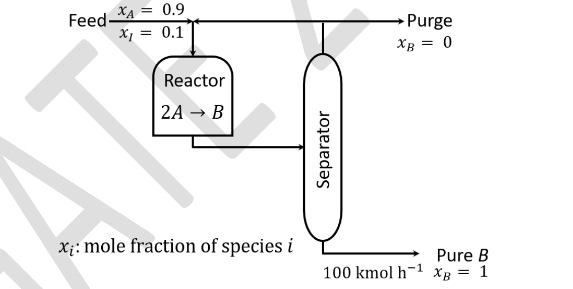
\includegraphics[width = 0.8\columnwidth]{q54}
		\caption*{}
		\label{fig:q54}
	\end{figure}
	
	\hfill{\brak{\text{GATE CH 2024}}}
	
	\item Methane combusts with air in a furnace as $CH_4 + 2O_2 \to CO_2 + 2H_2O$. The heat of reaction $\Delta H_{rxn} = -880$ kJ per mol $CH_4$ and is assumed to be constant. The furnace is well-insulated and no other side reactions occur. All components behave as ideal gases with a constant molar heat capacity of $44$ J mol$^{-1}\degree$C$^{-1}$. Air may be considered as $20$ mol\% $O_2$ and $80$ mol\% $N_2$. The air-fuel mixture enters the furnace at $50\degree$C. The methane conversion $X$ varies with the air-to-methane mole ratio, $r$, as $X = 1 - 0.1 e^{-2\brak{r-r_s}}$ with $0.9 r_s \le r \le 1.1 r_s$ where $r_s$ is the stoichiometric air-to-methane mole ratio. For $r = 1.05 r_s$, the exit flue gas temperature in $\degree$C, rounded off to 1 decimal place, is \underline{\hspace{2cm}}
	
	\hfill{\brak{\text{GATE CH 2024}}}
	
	\item An isolated system consists of two perfectly sealed cuboidal compartments A and B separated by a movable rigid wall of cross-sectional area $0.1$ m$^2$ as shown in the figure. Initially, the movable wall is held in place by latches $L_1$ and $L_2$ such that the volume of compartment A is $0.1$ m$^3$. Compartment A contains a monoatomic ideal gas at $5$ bar and $400$ K. Compartment B is perfectly evacuated and contains a massless Hookean spring of force constant $0.3$ N m$^{-1}$ at its equilibrium length \brak{\text{stored elastic energy is zero}}. The latches $L_1$ and $L_2$ are released, the wall moves to the right by $0.2$ m, where it is held at the new position by latches $L_3$ and $L_4$. Assume all the walls and latches are massless. The final equilibrium temperature, in K, of the gas in compartment A, rounded off to 1 decimal place, is \underline{\hspace{2cm}}
	\begin{figure}
		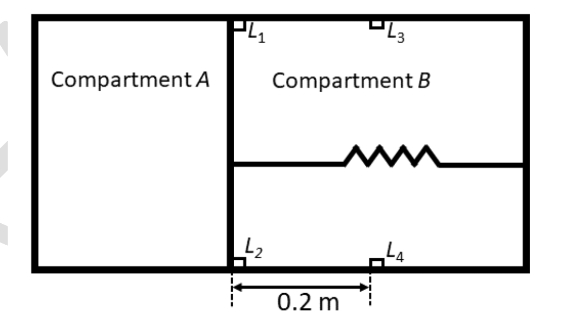
\includegraphics[width = 0.6\columnwidth]{q56}
		\caption*{}
		\label{fig:q56}
	\end{figure}
	
	\hfill{\brak{\text{GATE CH 2024}}}
	
	\item Ethylene obeys the truncated virial equation-of-state $\frac{PV}{RT} = 1 + \frac{BP}{RT}$ where $P$ is the pressure, $V$ is the molar volume, $T$ is the absolute temperature and $B$ is the second virial coefficient. The universal gas constant $R = 83.14$ bar cm$^3$ mol$^{-1}$K$^{-1}$. At $340$ K, the slope of the compressibility factor vs. pressure curve is $-3.538 \times 10^{-3}$ bar$^{-1}$. Let $G^R$ denote the molar residual Gibbs free energy. At these conditions, the value of $\brak{\frac{\partial G^R}{\partial P}}_T$, in cm$^3$ mol$^{-1}$, rounded off to 1 decimal place, is \underline{\hspace{2cm}}
	
	\hfill{\brak{\text{GATE CH 2024}}}
	
	\item A metallic spherical particle of density $7001$ kg m$^{-3}$ and diameter $1$ mm is settling steadily due to gravity in a stagnant gas of density $1$ kg m$^{-3}$ and viscosity $10^{-5}$ kg m$^{-1}$s$^{-1}$. Take $g = 9.8$ m s$^{-2}$. Assume that the settling occurs in the regime where the drag coefficient $C_D$ is inversely proportional to the Reynolds number, $\text{Re}$. The steady-state terminal velocity of the particle, in cm s$^{-1}$, rounded off to 1 decimal place, is \underline{\hspace{2cm}}
	
	\hfill{\brak{\text{GATE CH 2024}}}
	
	\item For the process flow diagram shown in the figure, the ratio of the purge to the fresh feed flow rate, rounded off to 2 decimal places, is \underline{\hspace{2cm}}
	\begin{figure}
		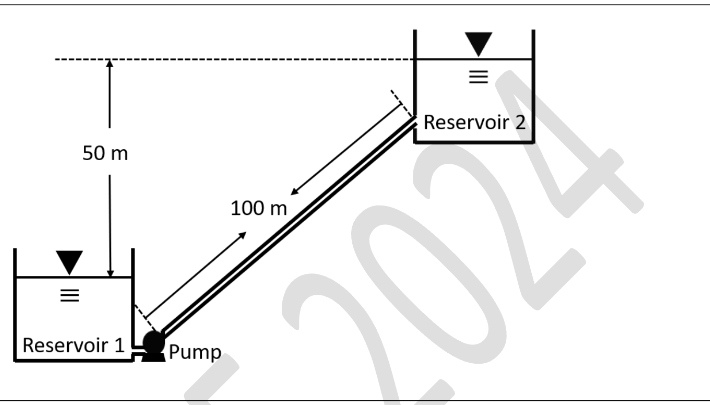
\includegraphics[width = 0.8\columnwidth]{q59}
		\caption*{}
		\label{fig:q59}
	\end{figure}
	
	\hfill{\brak{\text{GATE CH 2024}}}
	
	\item Consider the reaction $A \to B$ in a batch reactor. The reaction kinetics follow the rate law $-r_A = kC_A^{1.5}$ where $k = 0.1$ m$^{1.5}$ mol$^{-0.5}$ s$^{-1}$. The initial concentration of A is $10$ mol m$^{-3}$. The time, in s, required to reduce the concentration of A to $1$ mol m$^{-3}$, rounded off to the nearest integer, is \underline{\hspace{2cm}}
	
	\hfill{\brak{\text{GATE CH 2024}}}
	
	\item Consider the process in the figure with input $u$ and output $y$. The transfer function $G\brak{s}$ relates the output to the input as $G\brak{s} = \frac{y\brak{s}}{u\brak{s}}$. The magnitude of $G\brak{s}$ at a sinusoidal input frequency of $1$ rad s$^{-1}$, rounded off to 2 decimal places, is \underline{\hspace{2cm}}
	\begin{figure}
		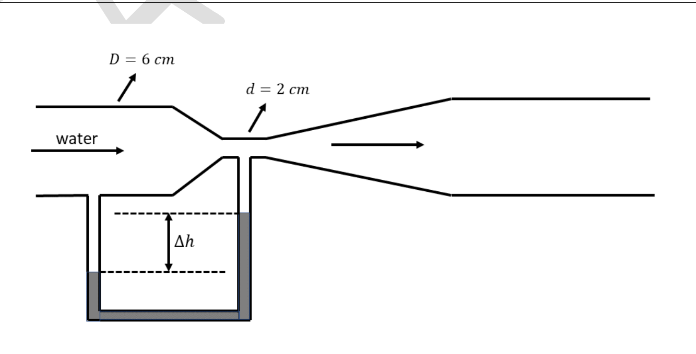
\includegraphics[width = 0.8\columnwidth]{q60}
		\caption*{}
		\label{fig:q61}
	\end{figure}
	
	\hfill{\brak{\text{GATE CH 2024}}}
	
	\item A pump is to be used for pumping $10$ m$^3$ min$^{-1}$ of water from an open tank to a large storage vessel. The water level in the storage vessel is $10$ m above the water level in the open tank. The frictional losses in the pipeline are given by $h_f = 10u^2$ where $h_f$ is in m and $u$ is the fluid velocity in m s$^{-1}$. The inner diameter of the pipe is $0.2$ m. The efficiency of the pump is $80\%$. The pump power, in kW, rounded off to 1 decimal place, is \underline{\hspace{2cm}} \brak{\text{Take acceleration due to gravity } g = 9.8 \text{ m s}^{-2}, \text{ density of water } \rho = 1000 \text{ kg m}^{-3}}
	
	\hfill{\brak{\text{GATE CH 2024}}}
	
	\item Consider the surge drum in the figure. Initially the system is at steady-state with a hold-up $\bar{V} = 5$ m$^3$, which is $50\%$ of full tank capacity, $V_{full}$, and volumetric flow rates $\bar{F}_{in} = \bar{F}_{out} = 1$ m$^3$ h$^{-1}$. The high hold-up alarm limit $V_{high} = 0.8 V_{full}$ while the low hold-up alarm limit $V_{low} = 0.2 V_{full}$. A proportional \brak{P-only} controller manipulates the outflow to regulate the hold-up $V$ as $F_{out} = K_c\brak{V - \bar{V}} + \bar{F}_{out}$. At $t=0$, $F_{in}$ increases as a step from $1$ m$^3$ h$^{-1}$ to $2$ m$^3$ h$^{-1}$. Assume linear control valves and instantaneous valve dynamics. Let $K_{c,min}$ be the minimum controller gain that ensures $V$ never exceeds $V_{high}$. The value of $K_{c,min}$, in h$^{-1}$, rounded off to 2 decimal places, is \underline{\hspace{2cm}}
	\begin{figure}
		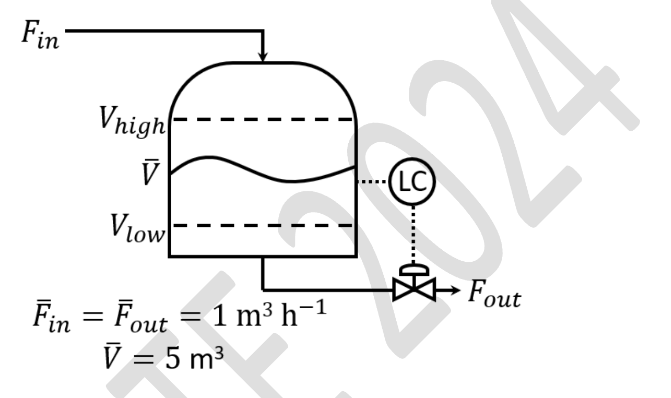
\includegraphics[width = 0.8\columnwidth]{q63}
		\caption*{}
		\label{fig:q63}
	\end{figure}
	
	\hfill{\brak{\text{GATE CH 2024}}}
	
	\item A PD controller with transfer function $G_c$ is used to stabilize an open-loop unstable plant with transfer function $G_p = \frac{1}{s-1}$. The control loop is a typical feedback loop with a negative feedback and a proportional gain of the measurement element of $1$. The minimum value of the proportional gain of the PD controller that ensures a stable closed-loop system is \underline{\hspace{2cm}}
	
	\hfill{\brak{\text{GATE CH 2024}}}
	
	\item The process of removing the fines from an ore by gravity separation using a stream of water is known as \underline{\hspace{2cm}}
	
	\hfill{\brak{\text{GATE CH 2024}}}
	
	\end{enumerate}
	
\end{document}
